%% For double-blind review submission
\documentclass[sigplan,10pt,review,anonymous]{acmart}
\settopmatter{printfolios=true}
%% For final camera-ready submission
%\documentclass[acmlarge]{acmart}\settopmatter{}

\makeatletter\if@ACM@journal\makeatother

%% Journal information (used by PACMPL format)
%% Supplied to authors by publisher for camera-ready submission
\acmJournal{PACMPL}
\acmVolume{1}
\acmNumber{1}
\acmArticle{1}
\acmYear{2017}
\acmMonth{1}
\acmDOI{10.1145/nnnnnnn.nnnnnnn}
\startPage{1}
\else\makeatother

%% Conference information (used by SIGPLAN proceedings format)
%% Supplied to authors by publisher for camera-ready submission
\acmConference[PL'17]{IEEE}{2018}{Planet Earh}
\acmYear{2017}
\acmISBN{978-x-xxxx-xxxx-x/YY/MM}
\acmDOI{10.1145/nnnnnnn.nnnnnnn}
\startPage{1}
\fi

\newcommand{\fer}[1]{\textcolor{red}{#1}}

%% For review submission
\setcopyright{none}

%% Bibliography style
\bibliographystyle{ACM-Reference-Format}
%\citestyle{acmauthoryear}

%% Packages that we are using in this version of the work:
\usepackage{amsmath}
\usepackage{hyperref}
\usepackage{paralist}
\usepackage{mathpartir}

% To turn comments OFF simply comment out the \Commentstrue line
\newif\ifComments\Commentstrue

\ifComments
\newcommand{\marcio}[1]{\noindent\textcolor{violet}{Marcio: {#1}}}
\newcommand{\guido}[1]{\noindent\textcolor{magenta}{Guido: {#1}}}
\newcommand{\fernando}[1]{\noindent\textcolor{brown}{Fernando: {#1}}}
\newcommand{\cesar}[1]{\noindent\textcolor{magenta}{Cesar: {#1}}}
\newcommand{\pedro}[1]{\noindent\textcolor{brown}{Pedro: {#1}}}
\newcommand{\rmv}[1]{\noindent\textcolor{gray}{Removed: {#1}}}
\newcommand{\new}[1]{\noindent\textcolor{blue}{ {#1}}}
\newcommand{\ed}[1]{\noindent\textcolor{red}{ {#1}}}
\else
\newcommand{\marcio}[1]{}
\newcommand{\guido}[1]{}
\newcommand{\fernando}[1]{}
\newcommand{\cesar}[1]{}
\newcommand{\pedro}[1]{}
\newcommand{\rmv}[1]{}
\newcommand{\new}[1]{#1}
\newcommand{\ed}[1]{}
\fi
\newcommand\dawn{\mbox{\textsf{DawnCC}}}
\newcommand\Taskminer{\mbox{\textsf{TaskMiner}}}

\newtheorem{Challenge}{Challenge}[section]

\begin{document}

\title[Automatic Identification and Annotation of Tasks in Structured
Programs]
{Automatic Identification and Annotation of Tasks in Structured Programs}

\author{Pedro Henrique Ramos Costa}
\authornote{with author1 note}          %% \authornote is optional;
\orcid{nnnn-nnnn-nnnn-nnnn}
\affiliation{
  \position{Researcher}
  \department{DCC}
  \institution{UFMG}
  \streetaddress{6627 Antonio Carlos Avenue}
  \city{Belo Horizonte}
  \state{Minas Gerais}
  \postcode{31.270-213}
  \country{Brazil}
}
\email{pedroramos@dcc.ufmg.br}

\author{Gleison Souza Diniz Mendonc\c{c}a}
\authornote{with author1 note}          %% \authornote is optional;
\orcid{nnnn-nnnn-nnnn-nnnn}
\affiliation{
  \position{Researcher}
  \department{DCC}
  \institution{UFMG}
  \streetaddress{6627 Antonio Carlos Avenue}
  \city{Belo Horizonte}
  \state{Minas Gerais}
  \postcode{31.270-213}
  \country{Brazil}
}
\email{gleison.mendonca@dcc.ufmg.br}

\author{Divino C\'{e}sar}
\authornote{with author1 note}
\orcid{nnnn-nnnn-nnnn-nnnn}
\affiliation{
  \position{Researcher}
  \department{IC}
  \institution{UNICAMP}
  \streetaddress{Cidade Universit\'{a}ria}
  \city{Campinas}
  \state{S\~{a}o Paulo}
  \postcode{13083-970}
  \country{Brazil}
}
\email{divcesar@gmail.com}

\author{Guido Ara\'{u}jo}
\authornote{with author1 note}
\orcid{nnnn-nnnn-nnnn-nnnn}
\affiliation{
  \position{Professor}
  \department{IC}
  \institution{UNICAMP}
  \streetaddress{Cidade Universit\'{a}ria}
  \city{Campinas}
  \state{S\~{a}o Paulo}
  \postcode{13083-970}
  \country{Brazil}
}
\email{guido@ic.unicamp.br}

\author{Fernando Magno Quint\~{a}o Pereira}
\authornote{with author1 note}
\orcid{nnnn-nnnn-nnnn-nnnn}
\affiliation{
  \position{Professor}
  \department{DCC}
  \institution{UFMG}
  \streetaddress{6627 Antonio Carlos Avenue}
  \city{Belo Horizonte}
  \state{Minas Gerais}
  \postcode{31.270-213}
  \country{Brazil}
}
\email{fernando@dcc.ufmg.br}          %% \email is recommended

\begin{abstract}
This paper reports the design and implementation of a suit of static analyses
and code generation techniques to annotate programs with OpenMP pragmas for
task parallelism.
These techniques approximate the ranges covered by memory regions, bound
recursive tasks and estimate the profitability of tasks.
We have used these ideas to implement a source-to-source compiler that inserts 
OpenMP pragmas into C/C++ programs without any human intervention.
By building onto the static program analysis literature, and relying on OpenMP's
runtime ability to disambiguate pointers, we show that we can annotate large and
convoluted programs, often replicating the performance gains of handmade
annotation.
Furthermore, our techniques give us the means to discover, without any 
development cost, opportunities of parallelism that remained buried in the syntax 
of well-known benchmarks for many years.
\end{abstract}

%% 2012 ACM Computing Classification System (CSS) concepts
%% Generate at 'http://dl.acm.org/ccs/ccs.cfm'.
 \begin{CCSXML}
<ccs2012>
<concept>
<concept_id>10011007.10011006.10011041</concept_id>
<concept_desc>Software and its engineering~Compilers</concept_desc>
<concept_significance>500</concept_significance>
</concept>
<concept>
<concept_id>10011007.10011006.10011008.10011024.10011035</concept_id>
<concept_desc>Software and its engineering~Procedures, functions and subroutines</concept_desc>
<concept_significance>300</concept_significance>
</concept>
<concept>
<concept_id>10003752.10003766.10003776</concept_id>
<concept_desc>Theory of computation~Regular languages</concept_desc>
<concept_significance>300</concept_significance>
</concept>
<concept>
<concept_id>10003752.10010124.10010131.10010134</concept_id>
<concept_desc>Theory of computation~Operational semantics</concept_desc>
<concept_significance>300</concept_significance>
</concept>
</ccs2012>
\end{CCSXML}

\ccsdesc[500]{Software and its engineering~Compilers}
\ccsdesc[300]{Software and its engineering~Procedures, functions and subroutines}
\ccsdesc[300]{Theory of computation~Regular languages}
\ccsdesc[300]{Theory of computation~Operational semantics}

\keywords{Parallelism, Tasks, OpenMP}

\maketitle

\section{Introduction}
\label{sec:intro}

Annotation systems have risen to a place of prominence as a simple and
effective means to write parallel programs.
Examples of such systems include OpenMP~\cite{JaegerCP15},
OpenACC~\cite{OpenACC20}, OpenHMPP~\cite{Andion14}, OpenMPC~\cite{Lee10},
OpenSs~\cite{MeenderinckJ11}, Cilk++~\cite{Leiserson09} and
Tareador~\cite{Ayguade15}.
Annotations work as a meta-language: they let developers grant parallel
semantics to syntax originally written to execute sequentially.
%\guido{What do you mean by modern accelerators? Not clear.}
Combined with modern hardware accelerators such as GPUs and FPGAs, they have led
to substantial performance gains~\cite{Bertolli14,Martineau16,Mendonca17,Poesia17,Reyes12,Antao16,Wienke12}.
%\guido{Suppport what?}
Nevertheless, although convenient, the use of annotations is not straightforward, 
and still lacks supporting tools that help programmers to check if annotations
are correct and/or effective.
%replaced:
%Yet, even if convenient,

%Annotations such as OpenMP or OpenACC still require developers to
%worry about typical hassles of the parallel world, such as race conditions
%and deadlocks.
%Moreover, because they are used in tandem with imperative programming languages,
%such troubles are only made worse by pointer aliasing.
There exist tools that insert automatic annotations in
programs~\cite{Amini12,Guelton12,Mendonca16,Pingali11,Nugteren14}.
All these technologies explore data-parallelism -- the possibility of running
the same computation independently on different data.
Another form of parallelism, based on tasks, remains still uncharted land in what
concerns automatic annotation.
Such fact is unfortunate, since much of the power of current annotation
systems lays on their ability to create tasks~\cite{Ayguade09}.
%\guido{Why the ability to create tasks makes such programs similar to irregular code?
%Which features of irregular code are resposible for such similarities? Not clear to the 
%reader}
As we illustrate in Section~\ref{sub:adv}, task parallelism -- the power to run
different routines simultaneously on independent data -- brings annotation systems
closer to irregular programs such as those that process graphs and
worklists~\cite{Ben-Nun17,Kulkarni11,Pingali11}.
The purpose of this work is to address this omission.

This paper describes \Taskminer, a source-to-source compiler that exposes task
parallelism in C/C++ programs.
To fulfil this goal, \Taskminer{} solves different challenges.
First, it finds program regions, e.g., loops or functions, that can be
effectively mapped onto tasks (Section~\ref{sub:identification}).
Second, it determines symbolic bounds to the memory blocks accessed within
those regions (Section~\ref{sub:sra}).
Third, it extracts parameters from the code to estimate when it is profitable to
create tasks.
These parameters feed conditional checks, which, at runtime, enable or disable
the creation of tasks (Section~\ref{sub:profit}) and limit their recursion
depth (Section~\ref{sub:ir}).
Fourth, \Taskminer{} determines which program variables need to be 
privatized in new tasks, or shared among them (Section~\ref{sub:variance}).
Finally, it maps all this information back into source code, producing
readable annotations (Section~\ref{sub:ir}).

In this paper, we defend the thesis that automatic task annotations are
effective and useful.
Our techniques enhance the productivity of developers, because they save them
the time to annotate programs.
\Taskminer{} receives as input C code, and produces, as output, a C
program annotated with human-readable OpenMP task directives.
We are currently able to annotate non-trivial programs, involving every
sort of composite type available in the C language, e.g., arrays, structs,
unions and pointers to these aggregates.
Some of these programs, such as those taken from the
Kastor~\cite{Virouleau14} or Bots~\cite{Duran09}
benchmark suites, are large and complex; thus, their manual annotation is a
time consuming and error prone task.
Yet, our automatically annotated programs not only approximate the execution
times of the parallel versions of those benchmarks, but are much faster than
\guido{Numbers?}
their sequential --unannotated-- versions, as we report in Section~\ref{sec:eval}.

\section{Challenges}
\label{sec:ovf}

This paper presents a tool that annotates source C code with OpenMP task
directives.
This tool uses novel techniques to fulfill its purpose.
Such techniques solve four challenges, which Section~\ref{sub:dif}
illustrates with examples.
However, before we dive into these challenges, the reader must understand
the main benefits of using a runtime environment such as OpenMP's, for
such advantages have guided most of our designing decisions.
Section~\ref{sub:adv} introduces this discussion.

\subsection{The OpenMP Runtime System}
\label{sub:adv}

The main advantage of using OpenMP annotations to split a program into parallel
tasks is
the ability  of leaving the job of  handling dependences to a runtime.
The OpenMP runtime maintains a task dependence graph which dynamically exposes more parallelism 
opportunities than those resulting from a conservative  compile-time  analysis.
In particular, the runtime lets us circumvent the shortcomings that pointer aliasing
impose on the automatic parallelization of code.
Aliasing -- the possibility of two pointers dereferencing the same
memory region -- either prevents parallelism altogether, or forces compilers to
resort to complex runtime checks to ensure its
correctness~\cite{Alves15,Ravishankar14}.
The OpenMP runtime shields us from this problem, because
it already checks for dependencies among tasks, and dispatches them in a
correct order~\cite{LaGrone11}.

Dependence tracking can be complex, involving checks over ranges of addresses
(if the runtime system treats dependencies across memory ranges).
It can also include memory labelling and renaming (if the
runtime system is able to remove false dependencies).
Regardless of its capacity -- which is not the same across every OpenMP
implementation -- the runtime system will represent dependencies using a task
dependence graph (TDG)~\cite{Duran08}.
In this directed acyclic graph, nodes denote tasks and edges represent
dependences between them.
Tasks are dispatched for execution according to a dynamic topological ordering of
this graph~\cite{Planas15}.

\begin{figure}[t!]
\begin{center}
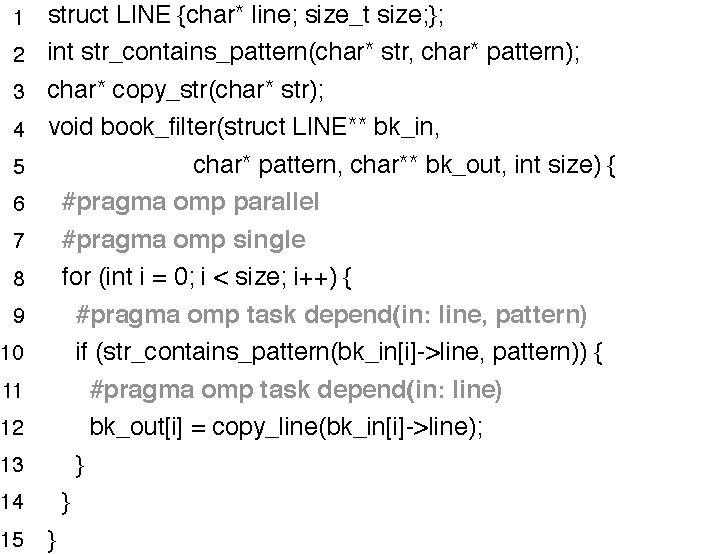
\includegraphics[width=1\columnwidth]{images/ex_book_filter}
\caption{The benefits of the OpenMP runtime environment.
Neither the runtime checks of Alves~\cite{Alves15} or Rus~\cite{Rus02}, nor
Whaley's context and flow sensitive alias analysis would be able to ensure the
correctness of the automatic parallelization of this program.}
\label{fig:ex_book_filter}
\end{center}
\end{figure}

OpenMP's runtime support allows the parallelization of irregular applications,
such as programs that traverse data-structures formed by a mesh of pointers.
In such programs, control constructs like {\tt if} statements make the
execution of some statements dependent on the program's input.
The runtime can capture such dependences, in contrast to static analysis tools.
As an example, Figure~\ref{fig:ex_book_filter} shows an application that
finds patterns in lines of a book\footnote{Whenever we show code, statements in
black font are part of the original program.
The annotations that we create automatically appear in grey.
The meaning of the pragmas used in the examples is explained in
Section~\ref{sec:sol}}.
The book is given as an array of pointers.
Each pointer leads to a string representing a potentially different line.
Out parallelization of this program consists in firing off a task
to process each line.
Figure~\ref{fig:ex_book_filter} has been annotated by
\Taskminer.
The OpenMP execution environment ensures the correct scheduling of the tasks
created at lines 9 and 11, by assuring that the annotated dependencies
{\tt line} and {\tt pattern}
are respected at runtime.

\subsection{Challenges}
\label{sub:dif}

As seen in Section~\ref{sub:adv}, the OpenMP runtime liberates us
from the burden of having to track dependences between pointers statically.
However, the automatic insertion of effective task annotations into
programs still required us to deal with a number of challenges.
If left unsolved, these challenges would restrict our interventions
to trivial annotations -- hardly be of any use.
Our first challenge is inherent to any automatic parallelization system.

\begin{Challenge}
\label{ch:Regions}
Identify the memory region covered by a task.
\end{Challenge}

\begin{figure}[b!]
\begin{center}
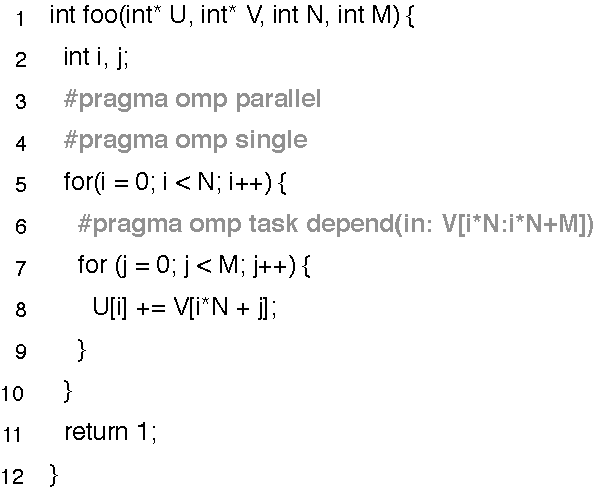
\includegraphics[width=1\columnwidth]{images/ex_Regions}
\caption{Challenges~\ref{ch:Regions} and~\ref{ch:cost}: identifying memory regions
with symbolic limits, and using runtime information to estimate the profit of
tasks.}
\label{fig:ex_Regions}
\end{center}
\end{figure}

Figure~\ref{fig:ex_Regions} illustrates Challenge~\ref{ch:Regions}, and shows
how we solve it.
That program receives an $\mathsf{M}\times\mathsf{N}$ matrix \textsf{V}, in
linearized format, and produces a vector \textsf{U}, so that \textsf{U[i]}
contains the sum of all the elements in line \textsf{i} of matrix \textsf{V}.
For reasons to be considered in Section~\ref{sub:identification},
our static analysis determines that each iteration of the outermost loops
could be made into a task.
Thus, tasks comprise the innermost loop, and traverse the memory region
between addresses $\textsf{\&V + i * N}$ and $\textsf{\&V + i * N + M}$.
The identification of such ranges involves the use of a symbolic algebra,
which we have borrowed from the compiler-related literature, as we
explain in Section~\ref{sub:sra}.
Figure~\ref{fig:ex_Regions} also introduces the second challenge that we
tackle:

\begin{Challenge}
\label{ch:cost}
Estimate the profitability of tasks at runtime.
\end{Challenge}

The creation of tasks involves a heavy runtime cost due to allocation,
scheduling and real-time management of the dependence graph
(see Sec.~\ref{sub:adv}).
Ideally, this cost should be paid only for tasks that perform an amount of work
sufficiently large to pay for their management.
Being an interesting program property, on Rice's sense~\cite{Rice53}, the amount
of work performed by a task cannot be discovered statically.
As we show in Section~\ref{sub:profit}, we can try to approximate this quantity, using,
to this end, program symbols, which are replaced with actual values at runtime.
For instance, in Figure~\ref{fig:ex_Regions}, we know that the body of the
innermost loop is formed by five instructions.
Thus, we approximate the amount of work performed by a task with the
expression \textsf{5 * M}.
We use the runtime value of \textsf{M} to determine, during the execution of the
program, if we create a task, or not.
Such test is carried out by the guard at line 7 of the figure, which is part of
OpenMP's syntax. Also, we provide a reliable estimate on the \emph{workload cutoff}
from which a task can be safely spawned without producing performance overhead.
This \emph{cutoff} considers factors such as number of available cores
and runtime information on the task dispatch cost in terms of machine
instructions. This is further explained in Section \ref{sub:profit}.

\begin{figure}[h!]
\begin{center}
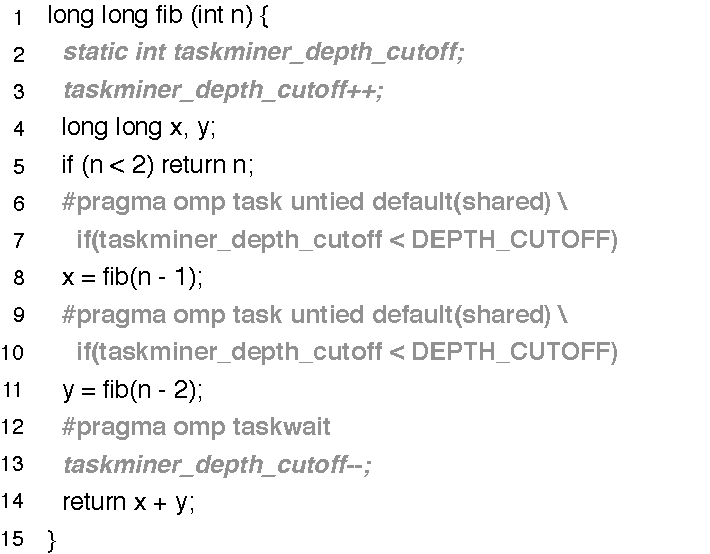
\includegraphics[width=1\columnwidth]{images/ex_cutoff}
\caption{Challenge~\ref{ch:cutoff}: bounding the creation of recursive tasks.
Example taken from~\cite[Fig.1]{Iwasaki16}.}
\label{fig:ex_cutoff}
\end{center}
\end{figure}

\begin{Challenge}
\label{ch:cutoff}
Bound the creation of recursive tasks.
\end{Challenge}

We introduce Challenge~\ref{ch:cutoff} by quoting Duran {\em et al.}:
``{\em In task parallel languages, an important factor for achieving a good
performance is the use of a cut-off technique to reduce the number of tasks
created}"~\cite{Duran08b}.
This observation is particularly true in the context of recursive, fine-grain,
tasks, as we analyze in Section~\ref{sub:ir}.
Figure~\ref{fig:ex_cutoff} provides an example.
To place a limit on the number of tasks simultaneously in flight, we associate
the invocation of recursive functions annotated with task pragmas with a
counter -- \textsf{taskminer\_depth\_cutoff} in Figure~\ref{fig:ex_cutoff}.
The guard in line 7 ensures that we never exceed \textsf{DEPTH\_CUTOFF}, a
predetermined threshold.
This example, together with Figure~\ref{fig:ex_Regions}, lets us emphasize that
the code generation algorithms presented in this paper are
parameterized by constants such as \textsf{DEPTH\_CUTOFF}, or
\textsf{WORK\_CUTOFF} in Figure~\ref{fig:ex_Regions}. Although these
have default estimates, we provide them as parameters to be set at will.

\begin{figure}[h!]
\begin{center}
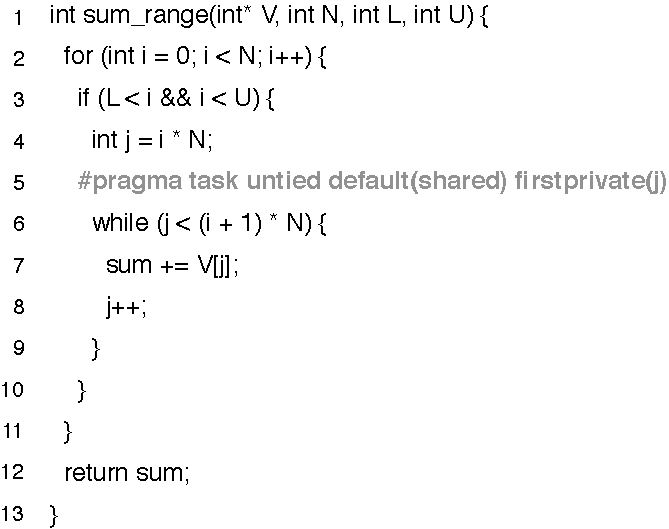
\includegraphics[width=1\columnwidth]{images/ex_privatize}
\caption{Challenge~\ref{ch:privatize}: variable \textsf{j} must be replicated among
tasks, to avoid the occurrence of data races.}
\label{fig:ex_privatize}
\end{center}
\end{figure}

\begin{Challenge}
\label{ch:privatize}
Identify private and shared variables.
\end{Challenge}

The two previous challenges are related to the performance of annotated
programs: if left unsolved, we shall have correct, albeit inefficient programs.
Challenges~\ref{ch:Regions}, and~\ref{ch:privatize}, in turn, are
related to correctness.
Challenge~\ref{ch:privatize} asks for the identification of variables that
must be replicated among threads.
This process of replication is called {\em privatization}.
As an example, variable \textsf{j} in Figure~\ref{fig:ex_privatize} must
be privatized.
In the absence of such action, that variable will be shared among all the
tasks created at line 5 of Figure~\ref{fig:ex_privatize}.
Because \textsf{j} is written within these tasks, race conditions would
ensue.
Section~\ref{sub:variance} explains how we distinguish private from
shared variables.

% The ability to handle pointers through speculative parallelization.

% when applied to general-purpose integer-intensive applications that have complex control flow and excessive pointer accesses, traditional parallelization tech- niques become quite ineffective, as they need to conservatively ensure program correctness by synchronizing all potential dependences in the program

% For example in 473.astar if we ignore dependences that only occur in less than 20% of all iterations, we can parallelize loops that correspond to 96% of total execution.

\section{Solutions}
\label{sec:sol}

Figure~\ref{fig:alg_main} provides a high-level view of a source-to-source
compiler that incorporates the techniques discussed in this paper.
The many parts of this algorithm shall be explained throughout this section.
This pseudo-code uses several concepts well-known in the compiler's
literature, such as control flow graphs~\cite{Kildall73} and
dependence graphs~\cite{Ferrante87}.
In the rest of this section we explain how we have combined this previous
knowledge to delimit and annotate tasks in structured programs.
Our presentation focus on the new elements that we had to add onto known
techniques, in order to adapt them to our purposes.

\begin{figure}[b]
\begin{center}
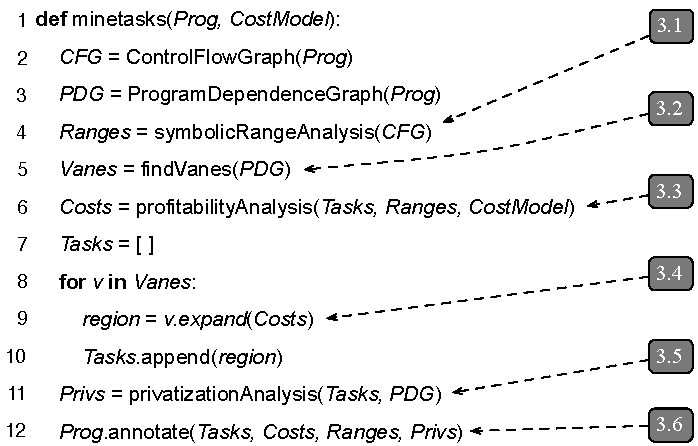
\includegraphics[width=1\columnwidth]{images/alg_main}
\caption{The main steps of our code generator.
Grey boxes show sections in this paper where each phase is discussed.}
\label{fig:alg_main}
\end{center}
\end{figure}

\paragraph{Tasks: syntax and scope:}
Our goal is to identify {\em tasks} in {\em structured} programs.
In the context of this work, a structured program is a program that can be
partitioned in {\em hammock regions}, a concept introduced by Ferrante
{\em et al.}~\cite{Ferrante87} in the middle 80's.
For completeness, we re-state it in Definition~\ref{def:hammock}.
Definition~\ref{def:task} formalizes the notion of task.

\begin{definition}[Hammock Region~\cite{Ferrante87}]
\label{def:hammock}
A Control Flow Graph $G$ is a directed graph with a starting node $s$, and an
exit node $x$.
A hammock region $G'$ is a subgraph of $G$ with a node $h$ that
{\em dominates}\footnote{A node $n_1 \in G$ dominates another node
$n_2 \in G$ if every path from  $S$ to $n_2$ goes across $n_1$.
Inversely, $n_1$ post-dominates $n_2$ if every path from $n_2$ to $x$ must
go across $n_1$.} the other nodes in $G'$.
Additionally, there exists a node $w \in G$, $w \notin G'$, such that
$w$ {\em post-dominates} every node in $G'$.
In this definition, $h$ is the {\em entry point}, and $w$ is the {\em exit point}
of $G'$.
\end{definition}

\begin{definition}[Task]
\label{def:task}
Given a program $P$, a task $T$ is a tuple $(G', M_i, M_o)$ formed by a hammock
region $G'$, plus a set $M_i$ of memory regions representing data that $T$ reads,
and a set $M_o$ of memory regions representing data that $T$ writes.
\end{definition}

Definition~\ref{def:task} uses the concept of {\em memory region}.
Syntactically, memory regions are described by program variables and/or pointers
plus ranges of dereferensable offsets.
Given two tasks: $T_1 = (G_1, M_{i1}, M_{o1})$ and $T_2 = (G_2, M_{i2}, M_{o2})$,
if $M_{o1} \cap M_{i2} \neq \emptyset$, then we say that $T_2$ {\em depends} on
$T_1$.
If a program $P$ is partitioned into a set of $n$ tasks, then this partition is
said to be {\em correct} if it abides by Definition~\ref{def:correctness}.

\begin{definition}[Correctness]
\label{def:correctness}
A set $T$ of $n$ tasks is a correct parallelization of a program $P$ if:
\begin{compactenum}
\item $T$ does not contain cyclic dependence relations;
\item the execution of the tasks in $T$ in any ordering determined by dependence
relations, leads to the same results as the sequential execution of $P$.
\end{compactenum}
\end{definition}

\begin{example}[Memory Regions]
\label{ex:regions}
Below we have two tasks, $T_{\mathit{foo}} = (\mathsf{foo}, \{\mathsf{v[i - 1]}\},
\{v[i]\})$ and $T_{\mathit{bar}} = (\mathsf{bar}, \{v[i]\}, \{\})$.
Dependencies are identified via the \textsf{depend} clause.
In this example, each hammock region is formed by one function call:
\end{example}

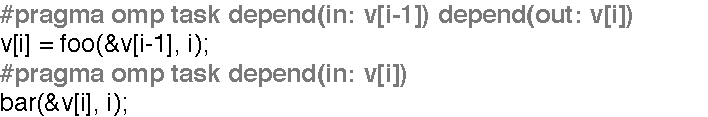
\includegraphics[width=1\columnwidth]{images/ex_depends}

\paragraph{The annotation zoo.}
Our equipment of choice to exploit task parallelism in programs is OpenMP 4.0.
%This annotation system lets us indicate to compiler
%and runtime environment when and how tasks must be created.
We describe below which annotations we are using, and explain, informally, their
semantics.
Full overviews of the syntax and semantics of these annotations is publicly
available\footnote{For a quick overview, we refer the reader to the leaflet
``Summary of OpenMP 4.0 C/C++ Syntax", which is made available by the OpenMP
group.}; hence, we shall not dive into their details.
%
\begin{compactitem}
\item \textsf{parallel} (\textit{clauses}): forms a team of threads
which will execute the marked program region in parallel.
\item \textsf{single} (\textit{clauses}): specifies that a
program region must be executed by one thread in the team.
\item \textsf{task} (\textit{clauses}): creates a new task.
\item \textsf{taskwait}: defines a synchronization point where
threads must wait for the completion of child tasks.
\end{compactitem}
%
Some pragmas are associated with lists of clauses.
There are several of these clauses available in OpenMP 4.0; however, we only use
the following:
\begin{compactitem}
\item \textsf{default([shared/private])}: indicates that variables are either
shared or replicated among tasks.
\item \textsf{firstprivate($v$)}: indicates that $v$ must be replicated among
tasks, and initialized with its value at the point where the annotation is
executed.
\item \textsf{untied}: if a task has this modifier, then its associated code can
be executed by more than one thread; e.g., threads might alternate execution due
to preemption and load balancing.
\item \textsf{depend}($\mathit{in}/\mathit{out}/\mathit{inout}$):
determine if data is read ($\mathit{in}$), written ($\mathit{out}$) or both
within a task region; thus, effectively setting dependences among tasks.
\item \textsf{if}({\em condition}): this clause defines the conditions
under which a task is allowed to create threads.
We use it to enforce the cost model.
\end{compactitem}

\subsection{Finding Symbolic Bounds of Arrays}
\label{sub:sra}

% Why this is necessary
To produce the annotations that create a task $T = (G, M_i, M_o)$, we need to
determine the memory regions $M_i$ that $T$ reads, and the memory regions $M_o$
that it writes.
Memory regions consist of pointers, plus ranges of addresses that these pointers
can dereference.
Example~\ref{ex:mem_reg} illustrates this notion.
To determine precise bounds to memory regions, we resort to an old ally of
compiler writers: the {\em Symbolic Range Analysis}, a concept that
Definition~\ref{def:sra} formalizes.

\begin{example}[Memory Region]
\label{ex:mem_reg}
The statement \textsf{U[i] += V[i*N + j]}, at line 9 of
Figure~\ref{fig:ex_Regions} contains two memory accesses: \textsf{U[i]} and
\textsf{V[i*N + j]}.
The first covers the memory region $[\mathtt{\&}\mathsf{U},
\mathtt{\&}\mathsf{U} + (\mathsf{M} - 1) \times \mathsf{sizeof}(\mathtt{int})]$.
The other covers the region
$[\mathtt{\&}\mathsf{V} + \mathsf{N} \times \mathsf{sizeof}(\mathtt{int}), \mathtt{\&}\mathsf{V} + ((\mathsf{i} \times \mathsf{M} + j) - 1) \times \mathsf{sizeof}(\mathtt{int})]$.
There is no code in Figure~\ref{fig:ex_Regions} that depends on the
loop in lines 8-10.
Thus, a task annotation must only account for the input dependence, e.g., the
access on \textsf{V}.
That is why the \textsf{depend} clause in line 6 contains a reference to this
region.
\end{example}

\begin{definition}[Symbolic Range Analysis]
\label{def:sra}
This is a form of abstract interpretation that associates
an integer variable $v$ with a {\em Symbolic Interval} $R(v) = [l, u]$, where
$l$ and $u$ are {\em Symbolic Expressions}.
A symbolic expression $E$ is defined by the grammar below, where $s$ is a
{\em program symbol}:
\renewcommand{\arraystretch}{0.9}
\[
\begin{array}{rcl}
E & ::= & z \ \ | \ \ s \ \ | E + E \ \ | \ \ E \times E \ \ | \ \  \mbox{min}(E, E) \ \ | \\
&  & \mbox{max}(E, E) \ \ | -\infty \ \ | \ \ +\infty
\end{array}
\]
\end{definition}

% How we do it.
The program symbols mentioned in Definition~\ref{def:sra} are names that cannot 
be reconstruct as functions of other names.
Examples include global variables, function arguments, and values returned by
external functions.
Symbolic range analysis is not a contribution of this paper: several
implementations of it exist.
We have adopted the one in the \dawn{} compiler~\cite{Mendonca17}, which, itself,
reuses work from Blume {\em et al.}~\cite{Blume94}.
The only extensions that we have added into \dawn's implementation was
the ability to handle C-like \textsf{structs}.
Therefore, we shall not provide further details about this part of our work.
To understand the rest of this paper, it suffices to know that this implementation
is sufficiently solid to handle the entire C99 language, always terminates, and
runs in time linear on the size of the program's dependence graph.
Thus, in the worst case, it is quadratic on the number of program variables.
If a program contains an array access $\textsf{V}[E]$, and we have that
$R(E) = [l, u]$, then the memory region covered by this access is, at least,
$[\mathtt{\&}\textsf{V} + l, \mathtt{\&}\textsf{V} + u]$.
The example below clarifies this observation.

\begin{example}
\label{ex:sra}
Symbolic range analysis, when applied onto Figure~\ref{fig:ex_Regions}, gives us
$R(\mathsf{i}) = [0, \mathsf{N} - 1]$, and $R(\mathsf{j}) = [0, \mathsf{M} - 1]$.
The memory access \textsf{V[i*N + j]} at line 9, when combined with this
information, yields the symbolic region that appears in the task annotation at
line 6 of Figure~\ref{fig:ex_Regions}.
\end{example}

\subsection{Mapping Program Regions to Tasks}
\label{sub:identification}

% Windmills and vanes
A {\em task candidate} is a set of program statements that can run in parallel
with the rest of the program.
To identify task candidates, we rely on the program's
{\em Dependence Graph}.
For completeness, Definition~\ref{def:pdg} revisits this notion.

\begin{definition}[Program Dependence Graph -- \cite{Ferrante87}]
\label{def:pdg}
Given a program $P$, its PDG contains one vertex for each statement $s \in P$.
There exists an edge from $s_1$ to $s_2$ if the latter depends on the former.
Statement $s_2$ is {\em data-dependent} on $s_1$ if it reads data that $s_1$
writes.
It is {\em control dependent} on $s_1$ if $s_1$ determines the outcome of a
branch, and depending on this outcome, we might execute $s_2$ or not.
\end{definition}

Task candidates are vanes in windmills.
{\em Windmills} are a family of graphs.
To the best of our knowledge, the term was coined by Rideau
{\em et al.}~\cite{Rideau08} to describe structural relations between register
copies.
Our windmills exist as subgraphs of the program's dependence graph.
We adopt a slightly more general definition than Rideaus'; however, the
metaphor that gave origin to the name: the shape of the graphs, is still
unmistakable:

\begin{definition}[Windmill -- \cite{Rideau08}]
\label{def:windmill}
A windmill is a graph $G_w = G_c \cup G_{v1} \cup \ldots \cup G_{vn}$ formed by
a strongly connected component $G_c$ (its center), plus $n$ components, not
necessarily strong, $G_{vi}$, the vanes, such that:
\begin{compactenum}
\item for any topological ordering of $G_w$, and nodes $n_c \in G_c$,
$n_v \in G_{vi}$, we have $n_c$ ahead of $n_v$;
\item for any $i$ and $j$, $1 \leq i < j \leq n$, $G_{vi}$ and $G_{vj}$ do not
share vertices (thus, sharing edges is also impossible).
\end{compactenum}
\end{definition}


\begin{figure}[h]
\begin{center}
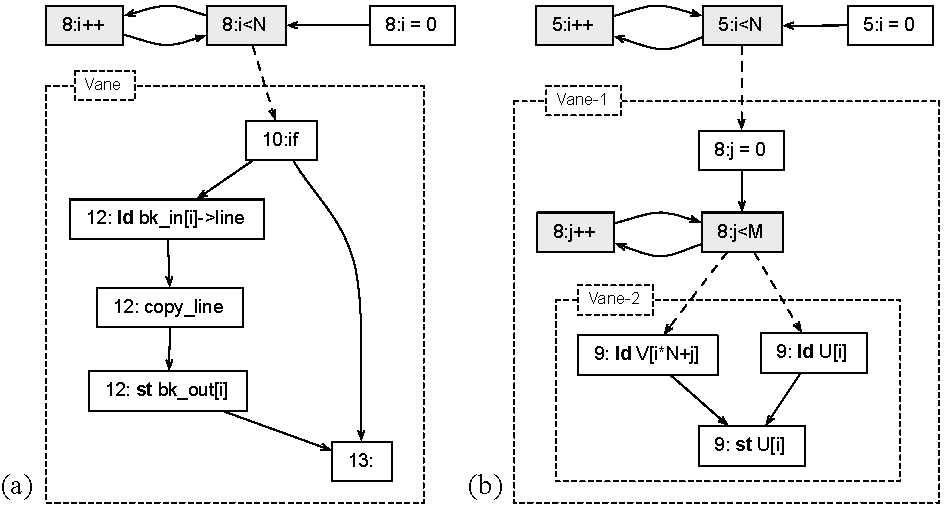
\includegraphics[width=1\columnwidth]{images/ex_windmill}
\caption{Examples of program dependence graphs.
Nodes that form centers of windmills are coloured in gray.
Data-dependence edges are solid; control-dependence edges are dashed.
Vanes of windmills appear within dotted boxes.
(a) PDG for Figure~\ref{fig:ex_book_filter};
(b) PDG for Figure~\ref{fig:ex_Regions}}
\label{fig:ex_windmill}
\end{center}
\end{figure}

Figure~\ref{fig:ex_windmill} shows two program dependence graphs, highlighting
windmills and their vanes.
The structure of windmills naturally leads to task candidates.
Vanes correspond to program parts that are likely to be executed
several times, because they sprout from a loop -- the center of the windmill.
Two different executions of the same vane can run in parallel.
This is a property of the PDG, and one of the original motivations behind its
design.
These two different executions can be seen as two instances of the same
structure (the vane), coming out of the same windmill center.
A topological ordering of the dependence graph does not impose any order among
these two hypothetical replicas of the same structure.

Windmills gives us structural properties to identify tasks.
We can find them via a depth-search traversal of the program's dependence
graph.
Function \textsf{findVanes}, in Figure~\ref{fig:alg_main} implements this
search.
However, not every windmill lead us to profitable tasks.
Furthermore, some windmills cannot be annotated, due to the inability of
range analysis to find bounds to the memory they access.
We deal with these shortcomings in the next two sections.

\subsection{Estimating the Profitability of Tasks}
\label{sub:profit}

% Explain the tension between large and small tasks.
The benefit of creating tasks depend on two factors:
runtime cost, and parallelism.
This tension leads to a sweet spot in the size of tasks, where size is
measured as the amount of code they execute.
The smaller the tasks are, the more parallel they tend to be, as a consequence
of less dependencies.
However, if tasks are too small, then the performance gained by the extra
parallelism might not compensate the cost of managing them.
On the other hand, if tasks are too big, then we might not obtain enough
parallelism, because individual tasks still execute sequentially.
In this paper, we mark as tasks {\em the first maximal analyzable vane above the
runtime cost}.
To imbue this last statement with meaning, in what follows, we define more
formally the notions of task size.
We leave the concept of maximal analyzable vane for Section~\ref{sub:expansion}.

\paragraph{Estimating the Size of Tasks.}
The size of a task is given by its workload, i.e., the number of instructions 
that such task executes.
The same program region might lead to the creation of tasks with different sizes.
Therefore, the actual size of a task is only known after it finishes execution.
However, to judge if the creation of a task is worth its cost, we must be able to
approximate its size statically.
With this goal, we define the notion of {\em Static Workload Estimate}:

\begin{definition}[Static Workload Estimate (SWE)]
\label{def:swe}
Let $G = G_1 \cup G_2 \cup \ldots \cup G_n$ be a partition of a program's control
flow graph $G$ into $n$ {\em disjoint} hammock regions.
We define the static workload estimate ($W(G)$) as a non-negative real number,
such that $W(G) = W(G_1) + W(G_2) + \ldots + W(G_n)$.
\end{definition}

Definition~\ref{def:swe} is too unconstrained: a function $W(G) = 0$ for any $G$
satisfies it.
However, we want $W$ to approximate the dynamic behavior of programs.
The literature contains heuristics to implement $W$.
Perhaps, the best-known among these heuristics is the static profiler of
Wu and Larus~\cite{Wu94}.
In this paper, we adopted a different approach: we reuse the symbolic range
analysis of Section~\ref{sub:sra} to augment static data with dynamic information.
In other words, we use symbolic range analysis to construct expressions that
represent the number of iterations of loops.
Similar approach has already been used to decide when to migrate virtual memory
pages in NUMA architectures~\cite{Piccoli14}.
OpenMP 4.0 contains syntax to enable the conditional creation of tasks.
Our symbolic analysis lets us build predicates for such conditional expressions.

\begin{example}
\label{ex:cond_task}
The condition in line 7 of Fig.~\ref{fig:ex_Regions} determines that tasks are
created if \textsf{5 $\times$ M $<$ WORK\_CUTOFF}.
\textsf{M} is a program symbol, i.e., a variable passed as argument to
function \textsf{foo}.
The expression \textsf{5 $\times$ M} is an approximation for the size of the
task that comprises the loop at lines 8-10.
The constant \textsf{WORK\_CUTOFF} represents the cost of creating a thread
in the OpenMP runtime, and it is determined empirically.
\end{example}

\begin{figure}[t!]
\begin{small}
\begin{eqnarray*}
\begin{tabular}{lc}
\textsc{[Instr]} &
W(\mbox{instr}) = \mbox{given by the spec.}
\\\\
\textsc{[Seq]} &
\inferrule{W(S_1) = w_1 \\ W(S_2) = w_2}{W(S_1;S_2;) = w_2}
\\\\
\textsc{[Branch]} &
\inferrule{W(S_1) = w_1 \\ W(S_2) = w_2 \\ W(S_3) = w_3}
{W(\mbox{if}(S_1) \ S_2; \ \mbox{else} \ S_3;) = w_1 + w_2 + w_3}
\\\\
\textsc{[LoopInf]} &
\inferrule{W(S_1) = w_1 \\ W(S_2) = w_2 \\ \mathit{Iter}(S_1) = \infty}
{W(\mbox{while} (S_1) \ S_2;) = 10 \times (w_1 + w_2)}
\\\\
\textsc{[LoopExp]} &
\inferrule{W(S_1) = w_1 \\ W(S_2) = w_2 \\ \mathit{Iter}(S_1) = E}
{W(\mbox{while} (S_1) \ S_2;) = E \times (w_1 + w_2)}
\end{tabular}
\end{eqnarray*}
\end{small}
\caption{\label{fig:swe}Estimating the cost of tasks.}
\end{figure}

% Explain how we use symbolic information to compute costs.
The declarative rules in Figure~\ref{fig:swe} sketches the heuristics that
we use to compute the SWE for a given hammock region $S$.
Rule \textsc{LoopInf} applies on loops whose number of iterations we cannot bound
via some symbolic expression computed statically.
Rule \textsc{LoopExp} represents loops that we can analyze using our Symbolic
Range Analysis.
The auxiliary function $\mathit{Iter}(S)$ returns a symbolic expression that
represents
the range of values covered by the code $S$ that controls the number of
iterations of the loop.
In Figure~\ref{fig:alg_main}, these rules are implemented by function
\textsf{profitabilityAnalysis}.

\paragraph{The Cost Model.}
A static workload estimate is only meaningful in the context of a {\em cost
model}.
A cost model is a collection of parameters that determine the impact of the
underlying computer architecture onto the creation and management of tasks.
The literature contains examples of techniques used to build cost models,
be it analytically~\cite{Baghsorkhi10}, or empirically~\cite{Poesia17}.
The automatic construction of a cost model is not the goal of this paper.
Instead, the reader shall notice that Figure~\ref{fig:alg_main} receives a
cost model as a parameter.
For the experiments in Section~\ref{sec:eval}, we have determined a small
collection of constants related to the creation of threads in our target
architecture, including the value of \textsf{WORK\_CUTOFF}, seen in
Example~\ref{ex:cond_task}.

% Discuss the expansion algorithm.
\subsection{Task Expansion}
\label{sub:expansion}

Task expansion consists in finding the smallest task that is large enough to
pay for the thread creation cost.
Figure \ref{fig:expand_alg} shows the algorithm that performs this activity.
We start this algorithm by setting \textsf{REGION} to be a hammock graph $H$
that corresponds to a vane within a windmill $W$.
The hammock decomposition of a structured program forms a tree~\cite{Ferrante87},
such that vertices in this tree represent hammock graphs.
$H_1$ is a child of $H_2$ in this tree if two conditions apply:
(i) $H_1 \subset H_2$, and (ii) for any 
other node $H_x$, if $H_1 \subset H_x$ then $H_2 \subset H_x$.
In this context, we call $H_2$ the {\em parent} of $H_1$.

\begin{figure}[h]
\begin{center}
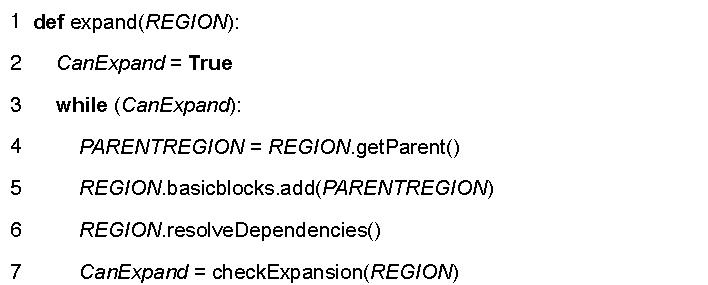
\includegraphics[width=1\columnwidth]{images/expand_alg}
\caption{Task discovery via expansion of hammock regions.
\textsf{COST} is the overhead of creating and scheduling threads.}
\label{fig:expand_alg}
\end{center}
\end{figure}

The routine \textsf{checkExpansion} sets the boolean \textsf{CanExpand} in
Figure~\ref{fig:expand_alg}.
This function is true as long as the following conditions apply:
(i) \textsf{VANE} has the structural properties of a
windmill's vane, i.e., it is contained within a windmill $W$;
(ii) we can analyze the memory regions within \textsf{VANE} using the
symbolic range analysis of Section~\ref{sub:sra};
(iii) \textsf{VANE} does not depend on another vane inside the same windmill $W$.

\begin{figure}[h]
\begin{center}
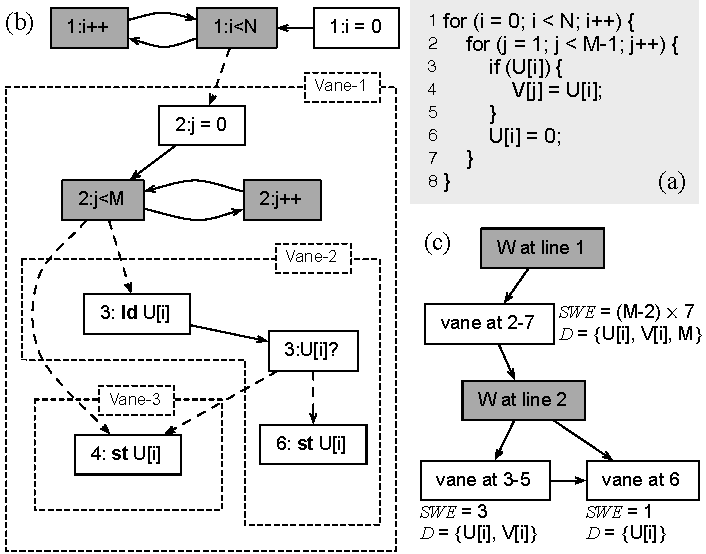
\includegraphics[width=1\columnwidth]{images/ex_expansion}
\caption{(a) Example of doubly nested loop that shall be analyzed by the 
\Taskminer.
(b) The dependence graph of the program.
(c) The decomposition of this loop into windmills and vanes.
$D$ is the set of variables the vane depends on.}
\label{fig:ex_expansion}
\end{center}
\end{figure}

The program in Figure~\ref{fig:ex_expansion} (a), a slight variation of
the code seen in Figure~\ref{fig:ex_Regions}, contains two windmills.
The first consists of the \textsf{for} loop at line 1.
The second, nested in the first, is the \textsf{for} loop at line 2.
The vanes that sprout from these windmills are highlighted in the program
dependence graph in Figure~\ref{fig:ex_expansion} (b).
The figure shows that we have three task candidates, each formed by a
different vane.
To find the actual tasks, we apply function \textsf{expand}
(Fig.~\ref{fig:expand_alg}) onto the innermost vanes: \textsf{Vane-2} and
\textsf{Vane-3}.
The latter cannot be expanded, as it depends on the former.
On the other hand, \textsf{Vane-2} can be expanded to include
\textsf{Vane-3}, as this expansion does not create new dependences between vanes
in the same windmill.

\noindent
\textbf{Rational:}
We expand tasks up to the \textsf{COST} threshold, which is determined
by the cost model seen in Section~\ref{sub:profit}.
If the profitability of a task is less than this constant, then parallelism
might not pay off the cost of managing threads.
However, if we expand tasks too much, then we might lose parallelism,
as code in a task runs sequentially.
Thus, determining \textsf{COST} is essential to the performance of our
optimization.
In this work, we have set this parameter empirically for the
runtime environment to be described in Section~\ref{sec:eval}.

\subsection{Privatization}
\label{sub:variance}

\Taskminer{} bestow a parallel semantics on code that has been originally
conceived to run sequentially.
This semantic gap might lead to race conditions.
Race conditions happen when annotations cause two or more threads to update
values that, in the sequential program, are denoted by the same name.
To avoid such situations, the insertion of annotations requires us to replicate
some values, making them private to each task.
We have named such replication {\em privatization}.

\begin{example}[Privatization]
\label{ex:priv}
Variables \textsf{i} and \textsf{j} in Figure~\ref{fig:ex_privatize} need to be
replicated among the tasks that the annotation at line 8 creates.
The need to replicate \textsf{j} is more apparent: this variable is updated in
the body of the task pragma, at line 9.
In the absence of replication, we have a race condition.
Variable \textsf{i} must also be replicated.
Each iteration of the loop at line 9 reads a different value of \textsf{i}.
Thus, each task should receive a different value in this variable.
In the absence of replication, all the threads would read the same value;  hence,
parallelization would change the semantics of the program.
\end{example}

\begin{definition}[The Private Requirement]
\label{def:private}
If a variable name has scalar type and contains at least one def-use chain that
enters the frontier of a task, then this name is said to bear the {\em private
requirement}.
The frontier of a task is determined by the \textsf{expand} function seen in
Figure~\ref{fig:expand_alg}.
\end{definition}

\begin{example}
\label{ex:priv_2}
Variable \textsf{i} must be privatized because it is defined at lines 2 and 10 of
Figure~\ref{fig:ex_privatize}, and is used at line 9 -- the body of a new task.
Moreover, this variable has a scalar type, e.g., \textsf{int}.
Similarly, variable \textsf{j} is defined at line 6, and is used at line 9.
This property -- the existence of def-use chains entering the task region --
leads to the insertion of the \textsf{firstprivate} clause at line 8 of
Figure~\ref{fig:ex_privatize}.
\end{example}

\noindent
\paragraph{firstprivate vs depend:} according to Definition~\ref{def:private},
only names representing scalar values are privatized.
These names have {\em value semantics}, i.e., they are ``passed
by copy" if used as actual arguments of functions.
Memory regions, that is to say, regions whose access happens through pointers,
are not privatized.
These regions are, instead, marked as dependences of the task, through the
\textsf{depend} clause.
Memory regions are discovered via the symbolic region analysis of
Section~\ref{sub:sra}.
In addition to pointers, we do not privatize values defined within
a task region, and used outside it.
That is to say: we privatize incoming def-use chains, but do not privatize
outgoing chains.
Values having this ``outgoing chain property" are shared by default.
We indicate this semantics via the \textsf{default(shared)} pragmas, as seen
in line 8 of Figure~\ref{fig:ex_privatize}.

\subsection{Mapping IR onto Source Code}
\label{sub:ir}

% Explain rational
The analyses described in Sections~\ref{sub:sra}-\ref{sub:variance} have
been implemented at the level of the LLVM intermediate representation.
We chose to implement those techniques at that level to benefit from the support
of several data-flow analyses already in place in the LLVM infra-structure.
In particular, this decision lets us reuse LLVM's scalar
evolution~\cite[p.18]{Grosser12}, from which we derive our symbolic analysis.
Additionally, we could reuse LLVM's program dependence graph, and its suite of
powerful alias analyses.
This toolbox gave us the necessary means to disambiguate pointers, albeit
conservatively, and estimate safe limits to memory regions.
However, our annotations are still inserted in C programs.
Having them in a high-level programming language has two main advantages:
they are human-readable, and thus can be debugged, and they are compatible with
compilers other than \textsf{clang}, such as \textsf{gcc}.
Thus, a major part of this work was the engineering effort to map
information from LLVM's intermediate representation back into C.

% Explain machinery: scope tree and simplification
\noindent
\textbf{The Scope Tree:}
To recover high-level information from the low-level IR, we have designed a
supporting data-structure henceforth named the {\em scope tree}.
The scope tree maps hammock regions into C constructions, such as
\textsf{while} and \textsf{if-then-else} blocks.
Each node of this graph represents a hammock region, augmented with
meta-information, such as the program part that it represents.
We keep track of these program parts via debugging information, which is
appended into the LLVM IR via the \textsf{-g} flag passed to the \textsf{clang}
compiler.
We have an edge from node $s_1$ to node $s_2$ if region $s_2$ is nested
within region $s_2$.
In the absence of control-flow optimizations such as loop unrolling or
dead-code elimination, each hammock region corresponds to some structured
code block (code region delimitable by braces).
Thus, we can find line numbers for each of the regions that we have marked
as tasks after the expansion seen in Section~\ref{sub:expansion}.

\noindent
\textbf{Simplification:}
before we annotate programs, we proceed to simplify these annotations.
Simplification happens via a system of rewriting rules, which explores 
identities.
Typical identifies include, for instance, $x + 0 = x$,
$\mathsf{max}(x, x) = x$ and $c \times \mathsf{max}(x, y) =
\mathsf{max}(c \times x, c \times y)$.
Identities are applied iteratively, until a fixed-point is reached.
Because we do not support commutativity, a fixed-point is guaranteed to be
always reached.
Notice that the source code that we produce is not totally equivalent to the
original program augmented with annotations.
To be able to insert annotations, we format the original code.
This operation involves, for instance, breaking lines containing multiple
statements, and inserting delimiting braces within every block in the program,
even one-liners.
This said, it is still possible that a task, after expansion, maps to a single
line that contains multiple statements, such as nested function calls.
In this case, we do not annotate the target program.
Section~\ref{sec:eval} provides data about \Taskminer's capacity to
annotate real-world programs.

\paragraph{Bounding Recursive Tasks}
During the evaluation of the \Taskminer, we observed that recursive
programs experienced performance regressions due to the excessive creation
of tasks.
To avoid this kind of slowdown, we currently give users the possibility to
bound the number of threads ever in flight, via a command line option, e.g.,
\textsf{./Taskminer -r 12} will limit the number of tasks to 12.
We implement this feature directly at the source code level, as part of the
final annotation of code.
Our solution is simple, yet, as the reader shall perceive in
Section~\ref{sec:eval}, it brings non-negligible benefits onto recursive
benchmarks.
Task bounding is implemented via a global variable, statically linked in the
program.
This variable is \textsf{taskminer\_depth\_cutoff} in Figure~\ref{fig:ex_cutoff}.
We insert code to increment it at the beginning of recursive functions that
are invoked within task regions, and we insert code to decrement it at each
return point of said functions.

\begin{example}[Task Bounding]
Figure~\ref{fig:ex_cutoff} illustrates the strategy that we
use to limit the number of tasks in flight due to recursive function
invocation.
The parameter \textsf{DEPTH\_CUTOFF} is determined by \Taskminer's users.
\end{example}

There are more involved ways to bound the number of tasks.
We believe that the state-of-the-art in the field today is the work of
Iwasaki and Taura~\cite{Iwasaki16,Iwasaki16B}.
These authors propose different techniques to limit the creation of tasks,
be it through the replication of code, be it through the estimation of work,
given function inputs.
Pragmas for the conditional creation of tasks, such as the one seen in
lines 7 and 10 of Figure~\ref{fig:ex_cutoff}, lets us obtain much of the benefit
of code versioning, as proposed by Iwasaki and Taura.
However, we found work estimation of recursive functions a task too difficult
to accomplish in general.
Quoting~\cite[p.355]{Iwasaki16}: ``{\em there are tasks which essentially do not
have simple termination conditions (e.g., tasks traversing pointer-based
trees)}".
Thus, although simple, our recursion counters are general enough, handling even
such tasks that are hard to bound symbolically.
Nevertheless, we still would like to explore further ways to cut-off extremely
fine-grained tasks in the future.

\section{Evaluation}
\label{sec:eval}
% In section 4. “Evaluation", subsection “Performance"; you state the only reason why programmers will strive for parallelism would be to achieve higher performance (faster program execution). I do not fully agree, and I believe we discussed that point earlier. There may be cases where performance of a single big core would be good enough to meet some target schedule (either response time or frame rate, etc.) still you may want to explore parallel versions of the code running on a cluster of smaller cores or a combination of a slow CPU and GPU to achieve better power efficiency.

% I believe this paper could be made stronger by also investigating the impact of power efficiency as a component of the cost function - if one looks at the latest processor chips from Intel and AMD, I can (finally) see there is a trend to increase the number of cores for all platforms.

% In the past there has been not much opportunity to take advantage of parallelism on 2 core platforms (especially notebook designs used to limit the number of real cores), but with 6 or 8 core processors entering the main stream, we may take advantage of running more processors slower (lower voltage) or spreading out the workload over a larger die area. It is quite interesting to note that running one core hot will increase the leakage in that area of the die much more (exponentially with temperature), so distributing work over a larger die area results in reduced leakage - having said that, a similar effect can be achieved by migrating the workload from core to core.

\noindent
\textbf{Runtime Environment:}
We have implemented the techniques described in this paper in
LLVM 3.9~\cite{Lattner04}.
All our experiments were performed in a 64-bits 12-core Intel(R) Xeon(R) CPU
E5-2620 at 2.00GHz, with 32K of L1 cache, 256K of L2 cache, 15M of L3 cache and
15Gb of main memory.
We use OpenMP 4.5, from November of 2015.

\noindent
\textbf{Research Questions:}
In this section, we evaluate this implementation, focusing on four research
questions:
%
\begin{compactitem}
\item \textsf{[Performance]}: how do our automatically annotated programs
compare against their sequential counterparts, or against manually annotated
versions?
\item \textsf{[Optimizations]}: what is the impact of the cost model
(Section~\ref{sub:profit}) and recursion bounding (Section~\ref{sub:ir}) onto
the programs that we annotate?
\item \textsf{[Versatility]}: how effective is \Taskminer{} in finding
opportunities to annotate general benchmarks?
\item \textsf{[Scalability]}: what is the runtime complexity of our
implementation of \Taskminer?
\end{compactitem}

\noindent
\textbf{Benchmarking:}
we have used different benchmarks in our experiments.
In Sections~\ref{sub:performance} and~\ref{sub:optimizations} we use
\textsf{BSC-Bots}\footnote{\url{https://github.com/bsc-pm/bots/tree/master/serial}} and \textsf{Swan}\footnote{\url{http://cuda.dcc.ufmg.br/swan/}}~\cite{Moreira17}.
In Section~\ref{sub:versatility} we use the LLVM test suite, and in
Section~\ref{sub:scalability} we use random programs produced with
\textsf{CSmith}~\cite{Yang11}.
Runtime numbers are averages of five executions.
We have not changed manually any of the benchmarks.

%PERFORMANCE
%Here, we show the results for our small benchmarks (toys & bots)
\subsection{Performance}.
\label{sub:performance}

\begin{figure}[htb]
\begin{center}
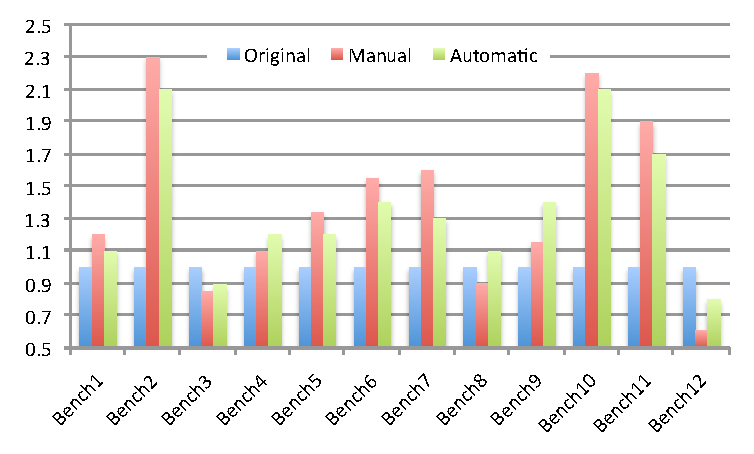
\includegraphics[width=0.9\columnwidth]{images/Absolute_speedups}
\caption{Speedup comparisons -- automatic annotations compare favourably against
manual interventions, and lead to great performance gains.
The Y-axis shows the speedup of either manual intervention, or automatic
annotation (this paper) onto the original programs.}
\label{fig:Absolute_speedups}
\end{center}
\end{figure}

%OPTIMIZATIONS
%Here, we show the results on two big optimizations: recursion depth and cost model.
%We can use the same benchmarks as above.
\subsection{Optimizations}.
\label{sub:optimizations}

\begin{figure}[htb]
\begin{center}
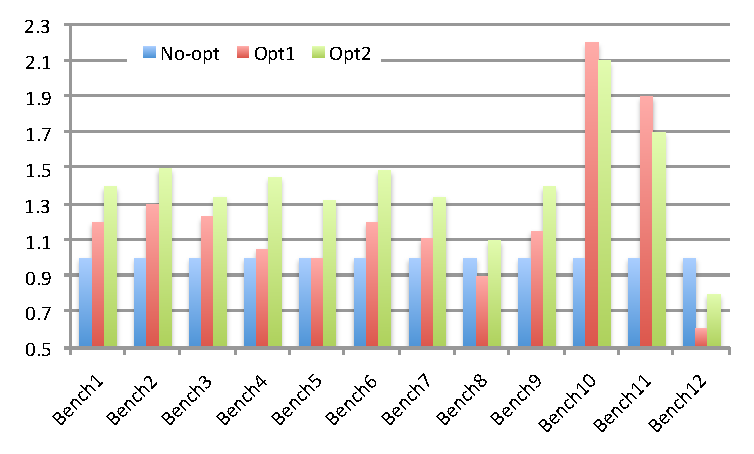
\includegraphics[width=0.9\columnwidth]{images/Opt_Speedups}
\caption{The benefit of our optimizations.
Each optimization (profitability analysis and recursion bounds) lead to
non-trivial speedups.}
\label{fig:Opt_Speedups}
\end{center}
\end{figure}

%VERSATILITY
%The goal here is to show that TaskMiner is a versatile tool, capable of finding many types of task parallelism in the code. 
%And the types of tasks that are going to be mined can be easily set, should the programmer ever desires to.
\subsection{Versatility}.
\label{sub:versatility}

\begin{table}[h]
\centering
\caption{Different kinds of tasks among the BOTS benchmarks. {\Taskminer}'s versaitily allows the user to define which type of tasks should be mined, annotated or cared for.}
\label{tab:types}
\begin{tabular}{|r|c|c|c|}
\hline
                   & \textbf{Recursive} & \textbf{FunctionCall} & \textbf{Region} \\ \hline
\textbf{fft}       & \checkmark         &                       & \checkmark      \\ \hline
\textbf{fib}       & \checkmark         &                       &                 \\ \hline
\textbf{floorplan} & \checkmark         &                       & \checkmark      \\ \hline
\textbf{sort}      & \checkmark         &                       & \checkmark      \\ \hline
\textbf{sparselu}  &                    & \checkmark            & \checkmark      \\ \hline
\textbf{strassen}  & \checkmark         &                       & \checkmark      \\ \hline
\textbf{uts}       & \checkmark         &                       &                 \\ \hline
\textbf{nqueens}   & \checkmark         &                       & \checkmark      \\ \hline
\textbf{knapsack}  & \checkmark         &                       & \checkmark      \\ \hline
\textbf{health}    & \checkmark         & \checkmark            & \checkmark      \\ \hline
\textbf{jacobi}    &                    &                       &                 \\ \hline
\end{tabular}
\end{table}


%APPLICABILITY
%We'll show TaskMiner application on larger benchmarks, such as those of spec or those of the LLVM's test-suite.
\subsection{Scalability}.
\label{sub:scalability}

\section{Related Work}
\label{sec:rw}

Mainstream compilers have only recently added support to OpenMP 4.0's task
parallelism.
An implementation of \textsf{clang} supporting tasks was released in March 14th,
2014\footnote{\url{https://clang-omp.github.io/}}.
A few weeks later, in April 22nd, 2014, such support was also announced in
\textsf{gcc} 4.9.
Thus, because the necessary infra-structure for the implementation of tasks is
relatively new, currently there are no tools, other than the \Taskminer,
that annotate programs automatically with these directives.
Nevertheless, there exists a long string of research aiming at the automatic
parallelization of programs.
In this section, we examine some elements in this list that relate to our
work.

Directive-based code annotation standards provide programmers with an easy-to-use
parallel programming model.
Task-based extensions to these standards have resulted in OpenMP 4.X,
StarSs \cite{bellens:sc:2006, perez:iccc:2008, planas:hpca:2009,
tejedor:hpdc:2011} and OmpSs \cite{bueno:icpp:2011, duran:ppl:2011}  which have
been extensively used to task-parallelize applications. Such
programming models come with tools that help programmers find the
best annotations for their code. For example,  Tareador
\cite{Ayguade15} enables a programmer, by means of a graphical interface,
to annotate sequential code, thus allowing the identification of potential task
parallelization opportunities.
Contrary to Tareador,  this paper proposes an approach that enables the
automatic insertion of OpenMP task annotations to relevant fragments of a
sequential program.

The techniques that we use to map program regions to tasks is similar to
analyses previously used in the generation of code for data-flow machines.
Data-flow programming was originally proposed as a candidate to enable
task-based parallelism \cite{agrawal:ipdps:2010, chan:spaa:2007,
gupta:micro:2011}.  Agrawal et al. \cite{agrawal:ipdps:2010}  extended
data-flow programming  with task input/output specifications in  Cilk++.
Vandierendonck et al.  \cite{vandierendonck:hotpar:2011} further extended Cilk++
with dependency clauses to facilitate the design of complex
parallelization patterns. Both groups presented a unified scheduler based on
fork-join parallelism \cite{vandierendonck:pact:2011} that enabled the
execution of task-based applications. Other approaches have also used
data-flow graphs to exploit parallelism, like Data-Driven Tasks
\cite{tasirlar:icpp:2011}, where the programmer can use put/await clauses to
determine task arguments before execution.
Function-based task parallelism was proposed by Gupta {\em et al.}
\cite{gupta:micro:2011} to use function arguments  as a way to
specify task  dependencies.
Notice that such research efforts focused on giving to programmers the tools to
{\em construct} parallel programs.
The automatic annotation of ordinary programs with data-flow constructs was not
among their goals.

Many systems have been developed to extract task parallelism from sequential
programs (semi) automatically.
Examples include OSCAR
(Optimally SCheduled Advanced multiprocessoR), Multigrain Parallelizing
Compiler \cite{ishizaka:journal:2000, kasahara:iwlcpc:2000},  MAPS (MPSoC
Application Programming  Studio) \cite{castrillon:tii:2013, ceng:dac:2008}, and
DiscoPoP (Discovery of Potential Parallelism) \cite{discopop, li:jss:2016}.
Besides parallelization systems, tools like Paraver \cite{extrae, paraver},
Aftermath~\cite{drebes:hipeac:2014}, DAGvis \cite{huynh:wvpa:2015}, and TEMANEJO
\cite{brinkmann:parco:2011, brinkmann:journal:2013, temanejo} were  designed to
enable performance analysis and visualization of task-based programs.
Although these tools help the programmer in adapting code
to run in parallel, they are not fully automatic.
For instance, the work that is the closest of ours, in reach and effectiveness,
in our opinion, is the suite of techniques proposed by Ravishankar {\em et
al.}~\cite{Ravishankar14}.
The type of irregular loops that they handle is impressive; however,
the lack of the runtime support \`{a} la OpenMP 4.X still requires them to
modify code before parallelization.
In their words: ``{\em For all benchmarks and applications, all functions were 
inlined, and arrays of structures were converted to structures of arrays for use
with our prototype compiler.}"

% Talk about annotations vs libraries, e.g., Wool, Intel TBB. See: "A Comparison of some recent Task-based Parallel Programming Models"

\section{Conclusion}
\label{sec:conc}

\pedro{As future work, we plan on performing Autotuning on {\Taskminer} to find good default parameters.
Autotuning works for data-flow applications have been already done in \cite{Trancoso17, Emani15}}.

\bibliography{references}

\end{document}
